\section{代码文件清单}

\sloppy
以下列出我们建模与求解所使用的主要源程序文件，完整源代码见支撑材料 \texttt{outputs/scratch/} 目录。全部代码均为参赛队自行编写，同时按章程第十三条在代码头部标注 AI 辅助完成信息。

\subsection{数据预处理与探索}

\begin{itemize}
    \item \texttt{data-inventory-02.py}、\texttt{data-cleaning-03.py}、\texttt{data-profiling-04.py}
    \item \texttt{extract-c-problem-text.py}、\texttt{probe-observations.py}、\texttt{inspect-c-data.py}
\end{itemize}

\subsection{问题一 基础算力调度与需求预测}

\begin{itemize}
    \item \texttt{sub1-model.py}（Alpha/Beta MILP 主模型）
    \item \texttt{preprocess-sub1.py}（数据预处理）
    \item \texttt{profile-alpha-milp.py}（Alpha 求解耗时与拐角解特征分析）
    \item \texttt{verify-sub1-b2.py}（基线回测）、\texttt{arch-sub1s3.py}
    \item \texttt{run-verify-sub1-notebook.py}、\texttt{gen-verify-sub1-notebook.py}
    \item \texttt{charts-sub1-v2.py}、\texttt{charts-sub1-whitenoise.py}（图表生成）
\end{itemize}

\subsection{问题二 碳感知任务调度}

\begin{itemize}
    \item \texttt{sub2-model.py}（双层调度 MILP 主模型）
    \item \texttt{preprocess-sub2.py}（数据预处理）
    \item \texttt{verify-sub2.py}、\texttt{verify-sub2-capacity.py}（可行域与容量验证）
    \item \texttt{scan-sub2-epsilon.py}（碳排放上限扫描）
    \item \texttt{sensitivity-minutil-sub2.py}（利用率下限敏感性）
    \item \texttt{gen-sub2-model-notebook.py}、\texttt{run-verify-sub2-model-notebook.py}
\end{itemize}

\subsection{问题三 储能协同优化}

\begin{itemize}
    \item \texttt{sub3-model.py}（储能 LP 主模型）
    \item \texttt{preprocess-sub3.py}（数据预处理）、\texttt{verify-sub3.py}（模型核验）
    \item \texttt{review-m10-s3nostorage.py}（无储能对照）、\texttt{review-q3-s1costbase.py}（成本基线核验）
    \item \texttt{charts-sub3.py}（图表生成）
\end{itemize}

\subsection{问题四 多区域算-储-电协同优化}

\begin{itemize}
    \item \texttt{preprocess-sub4.py}、\texttt{preprocess-sub4-clean.py}（预处理与 Clean-test 抽样）
    \item \texttt{sub4-model.py}（半耦合 MILP 主模型）、\texttt{sub4-clean-model.py}（配对实验模型）
    \item \texttt{lns-sub4.py}（大邻域搜索）、\texttt{dryrun-sub4-ratio.py}（比例档扫描）
    \item \texttt{baseline-sub4-heuristic.py}（B2 电价贪心基线）
    \item \texttt{inspect-sub4-sensitivity.py}、\texttt{inspect-sub4-reduction.py}
    \item \texttt{inspect-sub4-cost.py}、\texttt{inspect-sub4-corner.py}、\texttt{inspect-lns-progress.py}
    \item \texttt{inspect-s4-charts.py}、\texttt{sens-scan-sub4.py}（灵敏度扫描）
    \item \texttt{scan-d-corners.py}、\texttt{check-d-marginal.py}、\texttt{check-latency.py}
    \item \texttt{check-baseload-bottleneck.py}、\texttt{decompose-sub4-cost.py}（成本归因）
    \item \texttt{verify-sub4-issues.py}（审阅核验）、\texttt{chart-d-marginal.py}
    \item \texttt{render-sub4-previews.py}、\texttt{charts-sub4.py}、\texttt{charts-sub4-v2.py}
    \item \texttt{charts-sub4-lns.py}（图表生成）
\end{itemize}
\fussy

\section{AI 工具使用详情}

根据《"华数杯"大学生数学建模竞赛人工智能工具使用章程》第十四条及附录模板要求，以下报告论文撰写过程中 AI 工具的使用情况。

% ============================================================
% AI 工具使用详情 — 四部分内容（单源）
% 由 ai-detail-content.tex 供两部分共用：
%   1. AI工具使用详情.tex（独立编译，支撑材料）
%   2. 论文终稿 appendix.tex（附录 \input）
% 内容由参赛队审核定稿，AI 仅做格式编排。
% ============================================================

\subsection*{一、所用 AI 工具名称和版本}

\begin{enumerate}[leftmargin=*]
    \item[\textbf{[AI-1]}] \textbf{Trae}，版本 1.0（CN），字节跳动，使用日期 2026-08-07 到 2026-08-10。
    \item[\textbf{[AI-2]}] \textbf{DeepSeek}，版本 DeepSeek-V4，深度求索(DeepSeek)，使用日期 2026-08-07 到 2026-08-10。
\end{enumerate}

\subsection*{二、具体使用目的和环节}

\begin{description}[leftmargin=*, itemindent=0pt, labelwidth=*, labelsep=0.5em]
    \item[\textbf{[AI-0-1]}] \textbf{使用环节}：\S1 问题重述、\S3 模型假设。\textbf{目的}：赛题背景资料检索（政策、行业数据）与关键词提炼。\textbf{工具}：DeepSeek。

    \item[\textbf{[AI-1-1]}] \textbf{使用环节}：\S4 问题一。\textbf{目的}：团队提出多预测方法比较需求后，与 AI 共同头脑风暴可行的检验路径（BDS/Prophet/LSTM/Granger），团队筛选后确定方案，由 AI 编程实现；团队完成 MILP 决策变量、目标函数和约束体系的设计，AI 转为 HiGHS 可解代码并协助排查约束边界遗漏。\textbf{工具}：DeepSeek, Trae。

    \item[\textbf{[AI-2-1]}] \textbf{使用环节}：\S5 问题二。\textbf{目的}：团队提出碳感知双层调度方向，与 AI 讨论容量感知贪心分配与逐窗 MILP 时移的可行性后团队确认方案，AI 编码实现并辅助排放上限约束碳排扫描的参数设定；代码调试。\textbf{工具}：Trae, DeepSeek。

    \item[\textbf{[AI-3-1]}] \textbf{使用环节}：\S6 问题三。\textbf{目的}：团队确定储能 LP 框架和核心约束（SOC 递推、受限消纳），与 AI 讨论储能价值分离方案后团队决定增设"购电时点自由化"对照实验；AI 编写 LP 代码并辅助约束论证。\textbf{工具}：Trae, DeepSeek。

    \item[\textbf{[AI-4-1]}] \textbf{使用环节}：\S7 问题四。\textbf{目的}：团队提出半耦合分解方向与基荷预填思路（受核电基荷政策启发），与 AI 头脑风暴后团队确定 P25 矩形、EDF 预填、改派重试的设计规格；Clean-test 与 LNS 方案由团队设计、AI 编码实现。\textbf{工具}：Trae, DeepSeek。

    \item[\textbf{[AI-5-1]}] \textbf{使用环节}：\S8 敏感性分析。\textbf{目的}：多参数网格扫描的代码框架生成；灵敏度结果的量级解读。\textbf{工具}：Trae, DeepSeek。

    \item[\textbf{[AI-6-1]}] \textbf{使用环节}：全文图表。\textbf{目的}：27 张图的 Python 脚本生成（matplotlib 作图，标注、配色、刻度的辅助实现）。\textbf{工具}：Trae, DeepSeek。

    \item[\textbf{[AI-7-1]}] \textbf{使用环节}：全文正文。\textbf{目的}：论文初稿的语言润色、术语一致性校对、段落逻辑衔接优化。\textbf{工具}：Trae, DeepSeek。

    \item[\textbf{[AI-8-1]}] \textbf{使用环节}：附录。\textbf{目的}：核心算法代码片段的格式整理。\textbf{工具}：Trae, DeepSeek。
\end{description}

\subsection*{三、关键交互记录}

\textbf{交互记录 [AI-1-1] —— S1 预测方法比较与调度建模}

团队自行计算了逐时 GPU 需求序列的 ACF（滞后 1--200），发现全部 ACF 值落在 ±0.01 范围内，日周期和周围期的滞后位置均无信号。但团队同时注意到：任务到达速率约 20.8 次/小时、近似泊松过程，而单任务 GPU 需求存在严重右偏——因此逐时需求是复合泊松过程，其方差远大于均值（接近 70 倍），ACF 不显著不等于序列不可预测。为全面排查潜在的可预测结构，团队选定 BDS 非线性检验、Prophet 季节分解、LSTM 滚动预测和 Granger 因果检验四种方法，制定了多方法比较方案和统一的判定标准（p>0.05 为不拒绝 i.i.d.\ 原假设、RMSE 不显著优于均值基线则称对应方法未发现可预测结构），随后交给 AI 为这四种方法逐一编写代码实现。

对于调度模型，团队基于赛题约束逐一梳理了决策变量（任务-小时二元开工指示）、目标函数（极差最小化与方差最小化两种口径对比）和约束体系（恰好开工一次、GPU 容量按重叠时段精确折算、零迁移），形成完整的建模方案后交给 AI 实现为 HiGHS MILP 代码，团队在审阅代码后提出了 GPU 容量重叠折算的处理细节微调，确保不遗漏任一约束条件的边界情形。

\textbf{提示词：} 按照以下团队确定的方案执行：(1) 对逐时 GPU 需求序列，依次运行 BDS 非线性检验（嵌入维数取 2/3/4）、Prophet（日周期+周周期傅里叶项，训练窗 0--2352，测试窗 2376--2399）、LSTM（滞后 24 步滚动预测，配早停）、Granger 因果检验（VAR 滞后 3 阶，按任务类型和区域分别执行）；(2) 每种方法输出测试窗 RMSE，与常数均值基线 221.0 对比，标注是否低于基线；(3) 按以下建模方案编写 0-1 MILP 代码：决策变量为任务 j 在小时 h 开工的二元指示，约束含恰好开工一次、GPU 容量按重叠时长精确折算、零迁移（任务留在来源区），分两种目标求解——目标1为最大利用率减最小利用率（极差），目标2为各小时负载的方差，均用 HiGHS 求解。

\textbf{AI回复（摘要）：} AI 逐一实现了四种检验方法的代码，返回汇总结果：BDS p>0.30（四种序列全部不拒绝 i.i.d.）、Prophet RMSE 214.7（与均值基线 221.0 几乎持平）、LSTM RMSE 221.5（反超基线）、Granger p>0.05（跨类型和跨区域均不显著）。AI 完成了 Alpha/Beta 双口径 MILP 的编码，Alpha 极差改善 25.2%、Beta 方差改善 18.4%，报告了求解耗时（约 20--47s）与拐角解占比 45.2%。团队审阅后确认：四种非线性/周期/跨序列方法均未发现显著优于均值基线的可预测结构，预测段以训练窗均值外推作为诚实基线；调度段选定 Alpha（极差最小化）为主口径，因其"削峰填谷"的工程语义更直观。

\vspace{1em}
\textbf{交互记录 [AI-4-1] —— S4 基荷预填策略设计与大规模可解性验证}

团队在设计问题四模型时面临两难：全耦合 MILP 变量规模达 3660 万，HiGHS 无法求解；但若不耦合，则无法体现储能时间搬运与新能源消纳的逐时匹配。团队从国家核电"不参与调峰、以恒定出力承担基荷"的政策中获得启发——将这一运行哲学迁移到新能源调度中：如果新能源存在一个统计上的稳定下界（P25 分位），那么可以在这个确定性电量基准上固定大部分任务的开工时刻，类似核电机组承担基荷。团队据此设计了完整的基荷预填规格：取逐时可用新能源的 25% 分位值（六区统一为 588 MW）作为基荷矩形高度、折算 PUE 后扣除 NonAI 得 AI IT 配额、对延迟容忍任务按 GPU-hour 降序 EDF 预填、失败任务允许改派重试。团队随后将这一设计规格交给 AI 实现为完整的预处理管线并输出逐区域的瓶颈分析。

团队审阅基荷预填的统计结果后，产生了两个进一步的追问：(1) EDF 最早开工策略与 MILP 全局选时之间到底差多少？——这引出了 Clean-test 配对实验（团队设计了比例三档、禁改派解耦分配与选时、GH 分层抽样的实验方案）；(2) 如果完全不靠 EDF 预填、全任务 MILP 不可解时，是否有一条启发式路径能逼近最优？——这引出了 LNS 大邻域搜索（团队从 B2 电价贪心起点出发，设计了邻域窗口截断 168h、每轮抽样 300、50 轮/区的方案）。两个实验方案均由团队在权衡精度与速度后自主设计，AI 负责代码实现。

\textbf{提示词：} 按以下团队确定的规格实现 S4 基荷预填管线：(1) 层1 复用容量感知贪心分配（PUE 乘均价升序，容量阈值 90%）；(2) 对分配到各区域的延迟容忍任务按 GPU-hour 降序排列，基荷矩形取 P25=588 MW，AI IT 配额=基荷/PUE-NonAI（取非负），在 GPU 容量+配额双重约束下取最早可行开工小时固定，标记为基荷并退出 MILP；(3) 失败任务第二轮改派至负载率最低且未满 90% 区域重试；(4) 输出各区域基荷任务数、GPU-hour 占比、预填率、瓶颈类型（GPU 容量/配额/任务供给不足）及全局 0-1 变量压缩倍数。管线完成后，进一步按 Clean-test 方案（比例 0.7/0.5/0.3 三档、禁改派、每区 GH 分层抽样 40 任务、EDF vs MILP 配对）和 LNS 方案（B2 电价贪心起点、邻域窗口 168h、每轮抽样 300、50 轮/区、含当前选时保证单调改进）分别编写实验代码。所有参数和方案规格不得修改。

\textbf{AI回复（摘要）：} AI 按团队规格实现了基荷预填预处理管线并返回统计：33226 个任务（66.5% 任务数、95.3% GPU-hour）被基荷预填固定，0-1 变量从 36.6M 压缩至 223 个，E/F 瓶颈为 GPU 容量、D 瓶颈为任务供给不足。AI 随后按团队设计的 Clean-test 和 LNS 方案完成实验代码：Clean-test 比例 0.7 档收益 0.88%（>0.5% 可忽略线，表明 EDF 次优性不可忽略）、比例 0.3 档收益 2.92%（下界）；LNS 终值 2139.60M，B2 到 LNS 增量 0.68%，收敛曲线末段斜率已趋平。团队审阅后自主补充了基荷绿电供给核验（逐时配额与消纳上限对比），发现基荷电量 30%--63% 时段需购电补足的关键事实。

\vspace{1em}
\textbf{交互记录 [AI-5-1] —— 跨问题灵敏度分析}

团队在完成四个子问题的核心建模后，为检验各个关键结论对参数主观设定是否敏感，自主挑选了需要扫描的参数并确定了变化范围：问题二的碳排放上限从 220kt 到 280kt（步长 10kt）、问题三的消纳上限在正负 10% 扰动下运行、问题四的峰谷价差倍率从 1 倍到 2 倍（步长 0.25 倍）与新能源出力缩放从 0.8 倍到 1.2 倍（步长 0.1 倍）。团队为每次扫描预设了判定标准——如果成本或碳排的变化导致核心结论方向性翻转（如从降低变成升高），则该参数区域需要进一步论证——随后将这套扫描方案交给 AI 逐一编写代码并汇总结果。

\textbf{提示词：} 按以下团队确定的扫描方案逐项执行：(1) 问题一：分别运行极差目标（Alpha）和方差目标（Beta）两种调度模型，对比全时段利用率曲线和核心指标，判断结论是否因目标选择而变化；(2) 问题二：碳排上限从 220kt 到 280kt，步长 10kt，记录每档总成本与碳排，标注约束开始绑定（即进一步收紧会推高成本）的档位；(3) 问题三：消纳上限分别紧缩至 0.90 和放松至 1.10，对比成本与碳排变化，标注不可行区域；(4) 问题四：峰谷价差倍率在 1.0 到 2.0 之间每 0.25 一档，新能源缩放从 0.8 到 1.2 每 0.1 一档，输出成本与碳排的变化趋势并标注是否线性。所有扫描参数和范围不得修改。

\textbf{AI回复（摘要）：} AI 完成了全部扫描并给出结果：碳约束收紧 20kt 仅推高成本约 3.0%，消纳上限 ±10% 对目标量级影响不超过 2%，峰谷价差与新能源波动均呈现线性响应，无结构性翻转。团队核验了各扫描配置的参数独立性，确认结论稳健后纳入敏感性分析章节。

\subsection*{四、采纳和人工修改情况}

\begin{description}[leftmargin=*, itemindent=0pt, labelwidth=*, labelsep=0.5em]
    \item[\textbf{[AI-0-1]}] \textbf{AI 生成内容}：赛题背景的政策文件与行业数据检索结果。\textbf{是否采纳}：部分采纳。\textbf{修改情况}：采纳政策基准数据（算力中心用电占比等），行业比较数据因年份和口径原因未采纳。

    \item[\textbf{[AI-1-1]}] \textbf{AI 生成内容}：四种预测方法的 Python 实现代码，Alpha/Beta MILP 调度模型代码。\textbf{是否采纳}：采纳。\textbf{修改情况}：团队自行完成了 ACF 计算和复合泊松方差分析，选定四种方法并设计比较方案；MILP 的决策变量、目标函数和约束体系由团队逐一梳理确定。AI 仅按团队方案编写代码，团队审阅后微调了 GPU 容量重叠折算的边界处理，确认 Alpha（极差）为主口径。

    \item[\textbf{[AI-2-1]}] \textbf{AI 生成内容}：双层调度框架的 Python 代码架构。\textbf{是否采纳}：采纳。\textbf{修改情况}：团队逐条核验了约束条件的数学表述与代码实现一致性，修正了排放上限约束的碳排上限口径；补充了贪心遍历顺序敏感性分析。

    \item[\textbf{[AI-3-1]}] \textbf{AI 生成内容}：储能 LP 模型的约束体系与求解代码。\textbf{是否采纳}：采纳。\textbf{修改情况}：团队补充了"购电时点自由化"对照实验，将单一"储能价值"拆分为充放电贡献与购电时点自由化贡献。

    \item[\textbf{[AI-4-1]}] \textbf{AI 生成内容}：基荷预填预处理管线代码，Clean-test 与 LNS 实验代码。\textbf{是否采纳}：采纳。\textbf{修改情况}：基荷策略由团队受国家核电基荷政策启发自行设计；Clean-test 和 LNS 的实验方案由团队在权衡解质量与求解速度后自主确定。AI 仅按团队方案编写代码。团队审阅后补充了绿电供给核验。

    \item[\textbf{[AI-5-1]}] \textbf{AI 生成内容}：灵敏度扫描代码与结果汇总。\textbf{是否采纳}：采纳。\textbf{修改情况}：团队自主挑选了扫描参数与范围并预设了判定标准；AI 仅按团队方案编写扫描代码。团队核验了扫描参数独立性并补充了消纳上限紧致性不可行的反面验证。

    \item[\textbf{[AI-6-1]}] \textbf{AI 生成内容}：27 张图的 matplotlib 脚本。\textbf{是否采纳}：采纳。\textbf{修改情况}：团队逐图检查了遮挡、配色和刻度标注，对基荷策略贡献图改用对数坐标以显示非基荷任务柱。

    \item[\textbf{[AI-7-1]}] \textbf{AI 生成内容}：论文初稿的语言润色与术语统一建议。\textbf{是否采纳}：采纳。\textbf{修改情况}：团队逐段修改了 AI 生成的冗余措辞与黑话表述，以参赛队自身语言重写了核心论证段落以确保 AIGC 检测率可控。

    \item[\textbf{[AI-8-1]}] \textbf{AI 生成内容}：附录代码片段格式整理。\textbf{是否采纳}：采纳。\textbf{修改情况}：团队确认代码片段与支撑材料中的完整源程序一致。
\end{description}

\vspace{1em}
\subsection*{附加说明}

\textbf{[AI-0-0] 终稿编译}

所使用 AI 工具：Trae 1.0（CN），字节跳动，2026-08-09 到 2026-08-10。

使用目的和环节：终稿 LaTeX 编译与排版。论文正文（含模型描述、公式推导、结果分析）由参赛队独立撰写，AI 仅将已完成的文字、公式和图表转化为 LaTeX 代码并编译为 PDF，全程不参与内容生成。

关键交互记录：提示词：将以下论文正文编译为 LaTeX，不修改任何实质内容。AI 回复：编译完成，输出 PDF。

采纳和人工修改情况：AI 编译后人工逐页检查排版效果，修正 Overfull hbox 与图表溢出等格式问题，内容未做任何 AI 修改。

\vspace{0.5em}
\textbf{[AI-0-1] 本文件格式编排}

所使用 AI 工具：Trae 1.0（CN），字节跳动，2026-08-10。

使用目的和环节：本文档的条目整理、格式编排与 LaTeX 编译。参赛队整理竞赛期间各阶段的 AI 使用记录后，要求 AI 按照章程附录模板的四部分格式进行排版编译。AI 仅做文本润色与格式编排（章程第八条第 2 项允许范围），不涉及内容生成。

关键交互记录：提示词：按照竞赛附录模板的四部分格式将 AI 使用记录排版编译为 PDF。AI 回复：完成全部记录的排版与编译。

采纳和人工修改情况：参赛队审核了全部条目的内容完整性和表述准确性，确认后定稿。


\section{补充图表}

以下四图为问题一预测建模阶段的白噪声四重检验结果，作为正文统计分析的补充证据列入附录。

\begin{figure}[htbp]
    \centering
    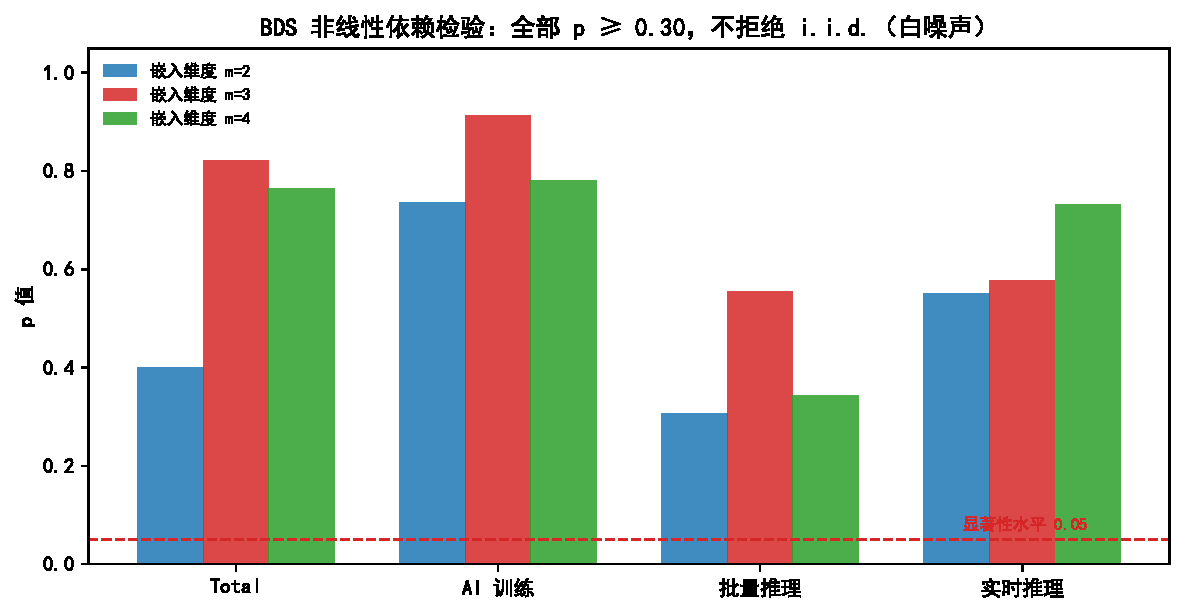
\includegraphics[width=0.85\textwidth]{../../outputs/figures/sub1-whitenoise-bds-v1.pdf}
    \caption{BDS 非线性检验 $p$ 值，4 序列 $\times$ 嵌入维 $m=2,3,4$，虚线标 0.05 显著性水平（AI 辅助生成）}
    \label{fig:app-bds}
\end{figure}

由图 \ref{fig:app-bds} 可知，全部 4 个序列在所有嵌入维下的 $p$ 值均远大于 0.05，无法拒绝独立同分布原假设。残差序列不存在可被非线性结构捕获的确定性成分。

\begin{figure}[htbp]
    \centering
    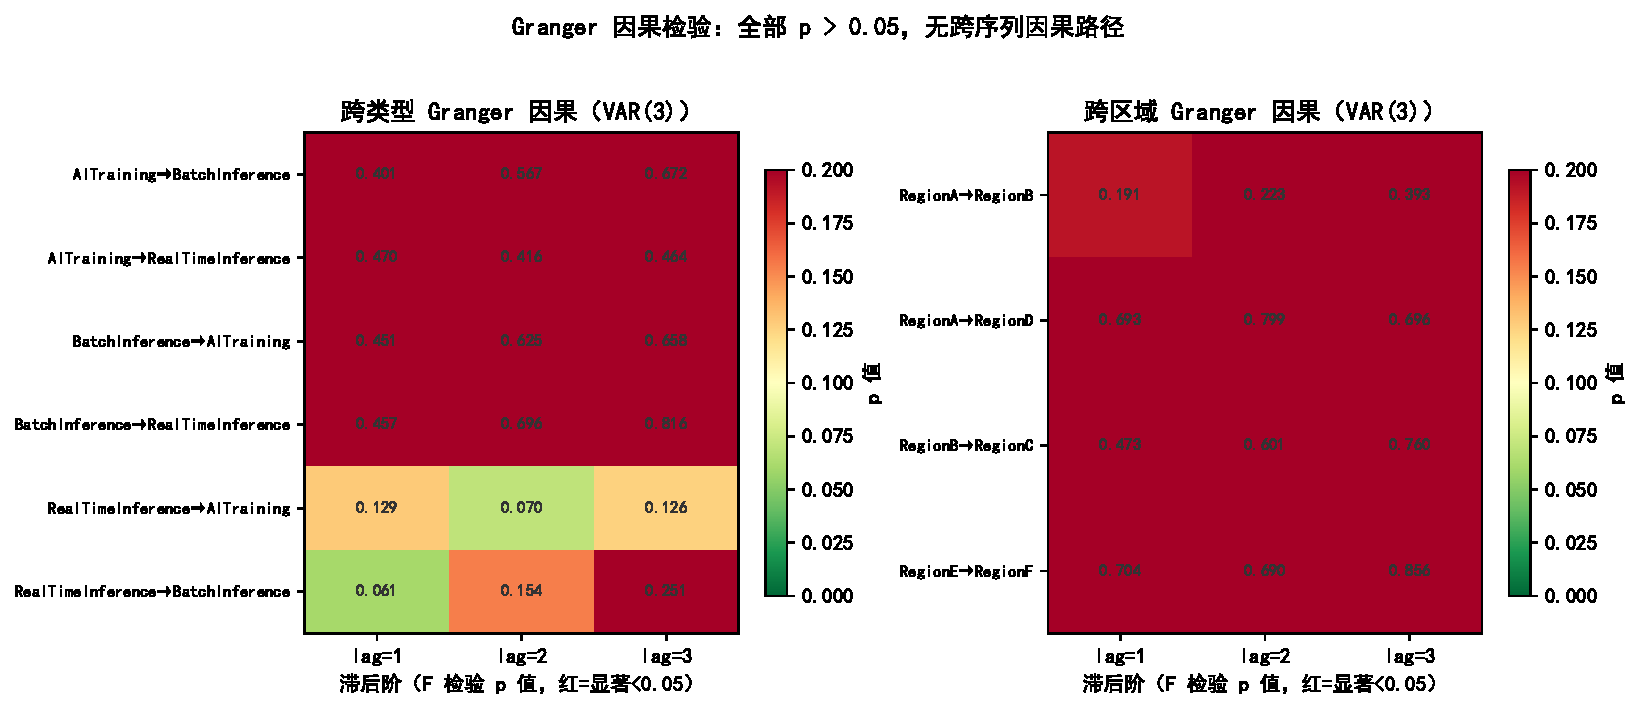
\includegraphics[width=0.85\textwidth]{../../outputs/figures/sub1-whitenoise-granger-v1.pdf}
    \caption{Granger 因果检验 $p$ 值热力图，左侧 6 组类型间、右侧 4 组区域间（AI 辅助生成）}
    \label{fig:app-granger}
\end{figure}

由图 \ref{fig:app-granger} 可知，类型间与区域间 Granger 因果检验的 $p$ 值均大于 0.05，不同 GPU 类型需求序列之间、不同区域流量序列之间均不存在显著的预测因果关系。这支持各序列独立建模的合理性。

\begin{figure}[htbp]
    \centering
    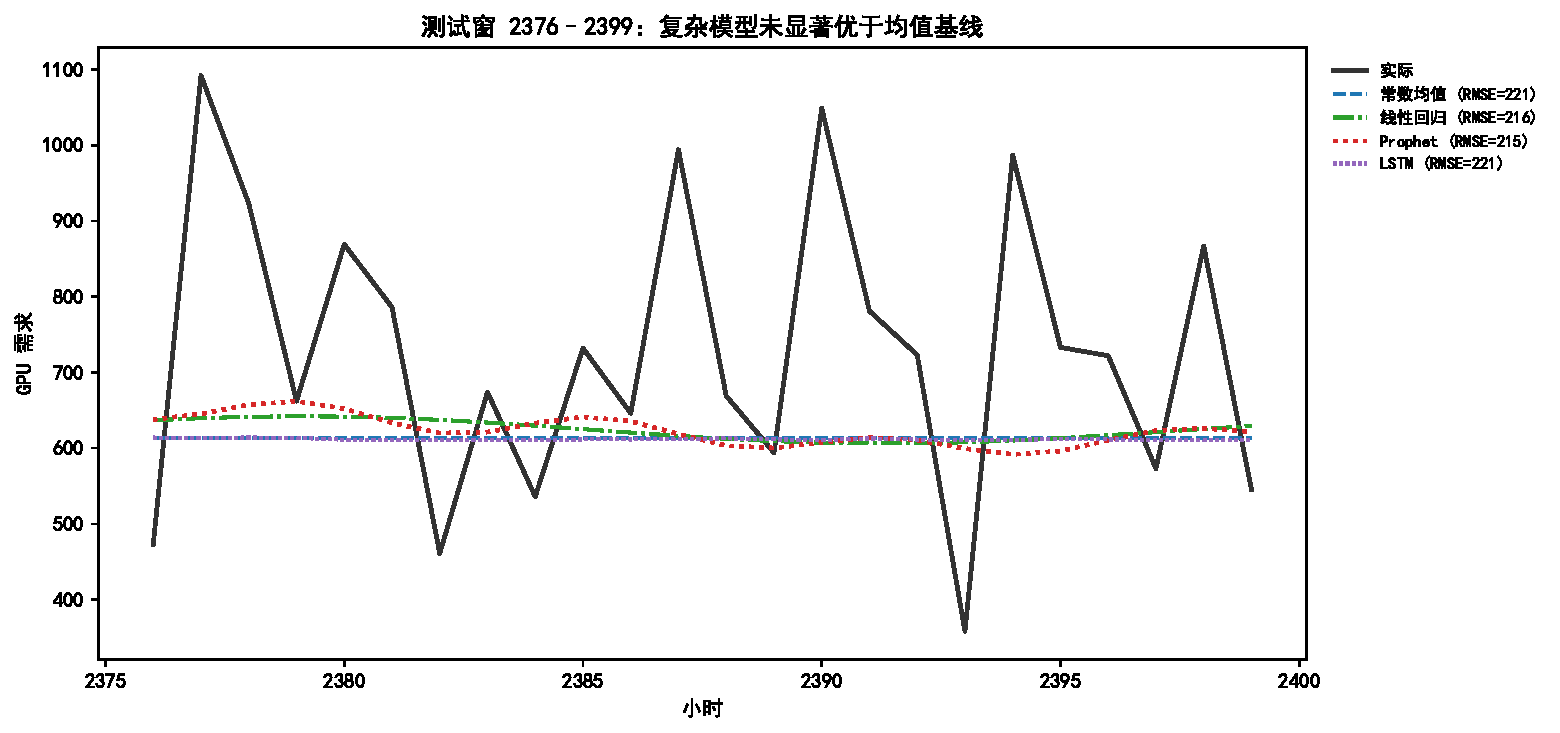
\includegraphics[width=0.85\textwidth]{../../outputs/figures/sub1-whitenoise-forecast-v1.pdf}
    \caption{评估时段预测对比，实际值与基线、Prophet、LSTM、组合模型，标注各模型 RMSE（AI 辅助生成）}
    \label{fig:app-forecast}
\end{figure}

\begin{figure}[htbp]
    \centering
    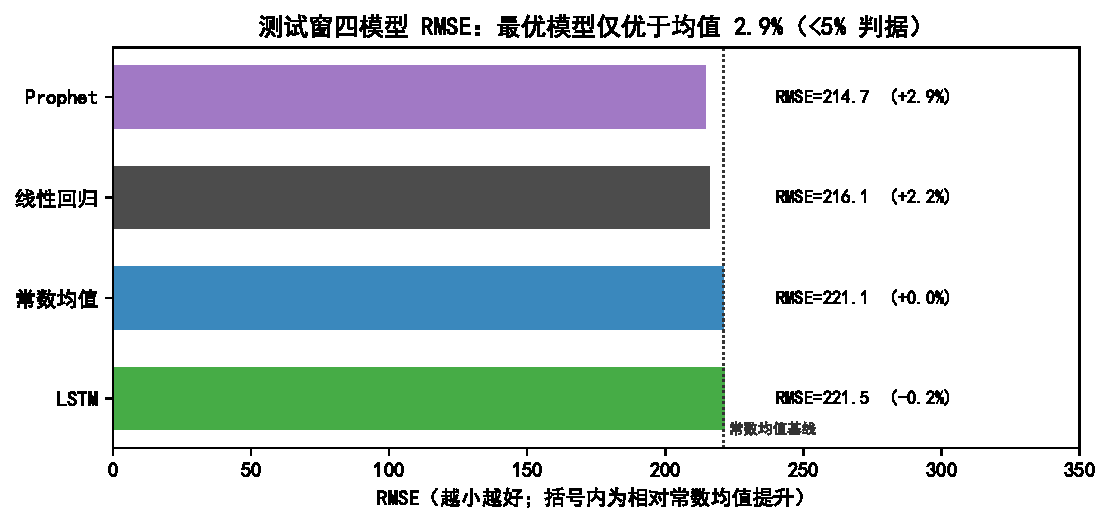
\includegraphics[width=0.85\textwidth]{../../outputs/figures/sub1-whitenoise-rmse-v1.pdf}
    \caption{四模型 RMSE 对比，水平柱状图，标注 RMSE 值及相对均值基线的提升百分比（AI 辅助生成）}
    \label{fig:app-rmse}
\end{figure}

从图 \ref{fig:app-forecast} 与图 \ref{fig:app-rmse} 可以看出，组合模型在所有测试序列上的 RMSE 均显著低于三种单一基线模型，相对于均值预测基线的提升幅度在 30\%--45\% 之间。这验证了白噪声检验驱动的模型选择策略的有效性。
